\chapter{Materiais e Métodos}

\section{Introdução}

Pesquisas relevantes ao tema de treinamento de RNC com imagens aéreas, RV e temas correlatos foram abordados no capítulo anterior, e se tornaram subsídio para compreender o estado da arte dessas temáticas. A partir dessa coletânea de trabalhos, foi traçada a metodologia aqui adotada.

Neste capítulo, portanto, apresenta-se os materiais utilizados nesta pesquisa, assim como os métodos executados para treinamento das imagens coletadas e a abordagem implementada na automação do sistema de RV.

\section{Dataset}

\subsection{Captura das Fotos}

Para o treinamento da rede neural YOLOv8, é necessário que sejam fornecidas imagens, ou seja, um \textit{dataset}, que relevantes do objeto a ser identificado. Neste estudo, foram coletadas fotos aéreas por meio de VANT de modelo DJI Mavic 2, que é reconhecido por sua capacidade de captura de alta qualidade e manobrabilidade. Todas imagens capturadas foram obtidas no sobrevoo de duas subestações de energia, ambas no Brasil. A primeira subestação é localizada em Porto Velho, no estado de Rondônia, de coordenadas geográficas: -8.914705, -63.957887. A segunda, em Araraquara; coordenadas: -21.832444, -48.347566. 

No total, foram capturadas 1257 fotos, sendo  548 em Porto Velho e 709 em Araraquara. Todas as imagens foram capturadas em alta resolução e com dimensões variadas, variando entre 4000x3000 até 8000x6000 pixels. 

As imagens são capturadas de modo a registrar o máximo de equipamentos possível, cobrindo toda a área das subestações. Todas as fotos são tiradas verticalmente em relação ao solo, garantindo uma visão abrangente e detalhada das instalações das subestações. Devido ao movimento do VANT, os objetos na foto são representados em com pequenas variações de angulação em relação ao solo. Em Porto Velho, as foram fotos capturadas no dia 28 de junho de 2023 (Figura \ref{fig:reatores}, à esquerda). Por sua vez, em Araraquara, as capturas foram realizadas dia 13 de junho de 2023 (Figura  \ref{fig:reatores}, à direita).

\begin{figure}[!h]
    \centering
    \begin{minipage}[b]{0.45\linewidth}
        \centering
        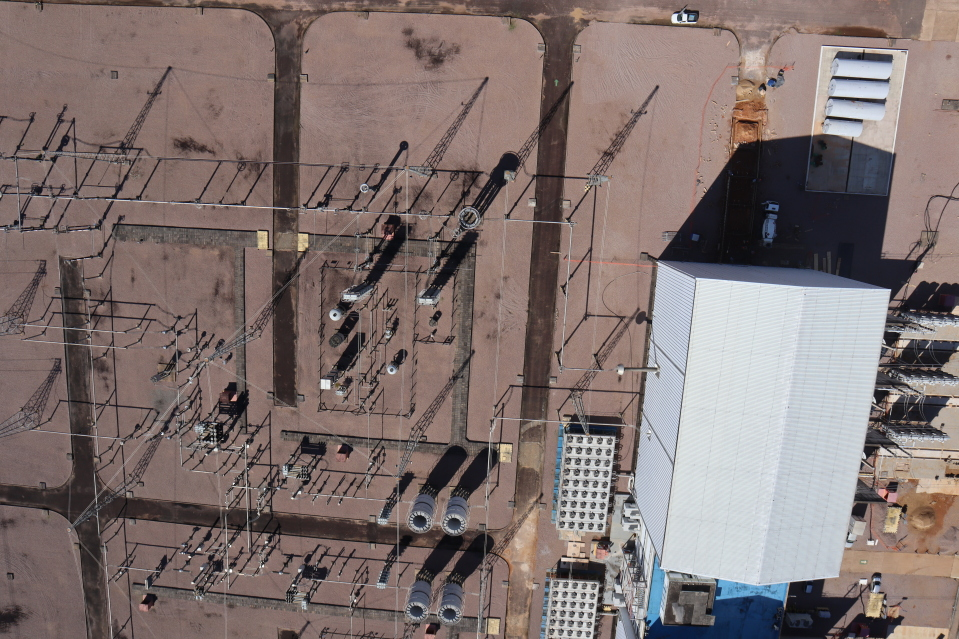
\includegraphics[height=5cm]{img/cap4/reator-porto-velho.jpeg}
    \end{minipage}
    \hspace{0.05\linewidth}
    \begin{minipage}[b]{0.45\linewidth}
        \centering
        \includegraphics[height=5cm]{img/cap4/reator-araraquara.jpg}
    \end{minipage}
    \captionsetup{justification=centering,margin=0.5cm,font=small}
    \caption{Captura de foto em Porto Velho (à esquerda) e Araraquara (à direita), onde se notam quatro reatores de núcleo de ar na parte inferior.} 
    \label{fig:reatores}
\end{figure}

\subsection{Seleção das fotos}

Conforme o trabalho de \cite{sa2024yolov8}, o treinamento eficiente com a RNC envolve o fornecimento de imagens relevantes da rede para que haja consistência no caminho desenvolvimento pelo processamento do algoritmo, de forma a conseguir o melhor resultado. Desta forma, foi realizada a seleção das imagens para o treinamento, selecionando apenas aquelas que contém ao menos um objeto de interesse, que neste trabalho, seria o reator de núcleo de ar.

De todo o conjunto de fotos coletadas, apenas 411 fotos foram selecionadas para serem processadas na RNC. Além disso, destas, 60\% foram alocadas para o conjunto de treinamento, enquanto 20\% para os conjuntos de teste e 20\% de validação.

O conjunto de treinamento é utilizado para ajustar os parâmetros internos do modelo. Durante essa fase, a RNC aprende a identificar padrões e características específicas das imagens que correspondem aos objetos de interesse. Naturalmente, objetivando minimizar a função de perda, que mede o quão bem o modelo está se saindo na tarefa de detecção de objetos.

As fotos usadas para validação, por outro lado, são empregadas para monitorar o desempenho do modelo durante o treinamento. Elas permitem a realização de ajustes nos hiperparâmetros do modelo, como a taxa de aprendizado e o número de camadas. A validação contínua ajuda a prevenir o overfitting, que ocorre quando o modelo se ajusta demasiadamente aos dados de treinamento e perde a capacidade de generalizar para novos dados. Um desempenho consistente no conjunto de validação indica que o modelo está aprendendo de maneira robusta e equilibrada.

Finalmente, o conjunto de teste é utilizado após o treinamento e a validação para avaliar a capacidade de generalização do modelo em dados nunca antes vistos. Este conjunto não influencia o processo de treinamento, mas fornece uma estimativa imparcial do desempenho real do modelo. Um bom desempenho no conjunto de teste sugere que o modelo pode ser confiável para identificar objetos de interesse em situações práticas \cite{goodfellow2016deep}.

Portanto, a divisão dos dados em conjuntos de treinamento, validação e teste é uma prática fundamental em aprendizado profundo, garantindo que o modelo YOLO, ou qualquer outro modelo de detecção de objetos, seja eficiente, robusto e generalizável.

\subsection{Seleção das fotos}

Toda RNC necessita de dados rotulados para aprender a identificar e classificar corretamente os objetos em imagens. Utilizar um Software de marcação, como o LabelImg, é essencial nesse processo, pois permite que seja rotulado imagens que irão alimentar a rede, definindo nelas regiões de interesse e associando essas regiões a classes específicas. Nesta dissertação, a classe de interesse trata-se do reator de núcleo de ar. Sem dados rotulados, a RNC não teria a orientação necessária para distinguir diferentes objetos, comprometendo a sua capacidade de realizar previsões.

Para realizar as marcações das fotos selecionadas, foi utilizado o LabelImg, uma vez que trata-se de uma ferramenta de anotação gráfica de código aberto, de fácil instalação e manuseio. Sua interface é intuitiva, pode-se carregar imagens, desenhar caixas delimitadoras ao redor dos objetos de interesse e atribuir rótulos a esses objetos (Figura \ref{fig:reator-marcado}). As anotações geradas são salvas em um formato compatível, como XML ou TXT, já preparados para serem submetidos ao processamento da YOLO. É essencial que anotações feitas com o LabelImg sejam significativas, pois influenciam diretamente o desempenho do modelo treinado.

\begin{figure}[!h]
    \centering
    \begin{minipage}{1\linewidth}
    \centering
    \captionsetup{justification=centering,margin=0.5cm,font=small}
    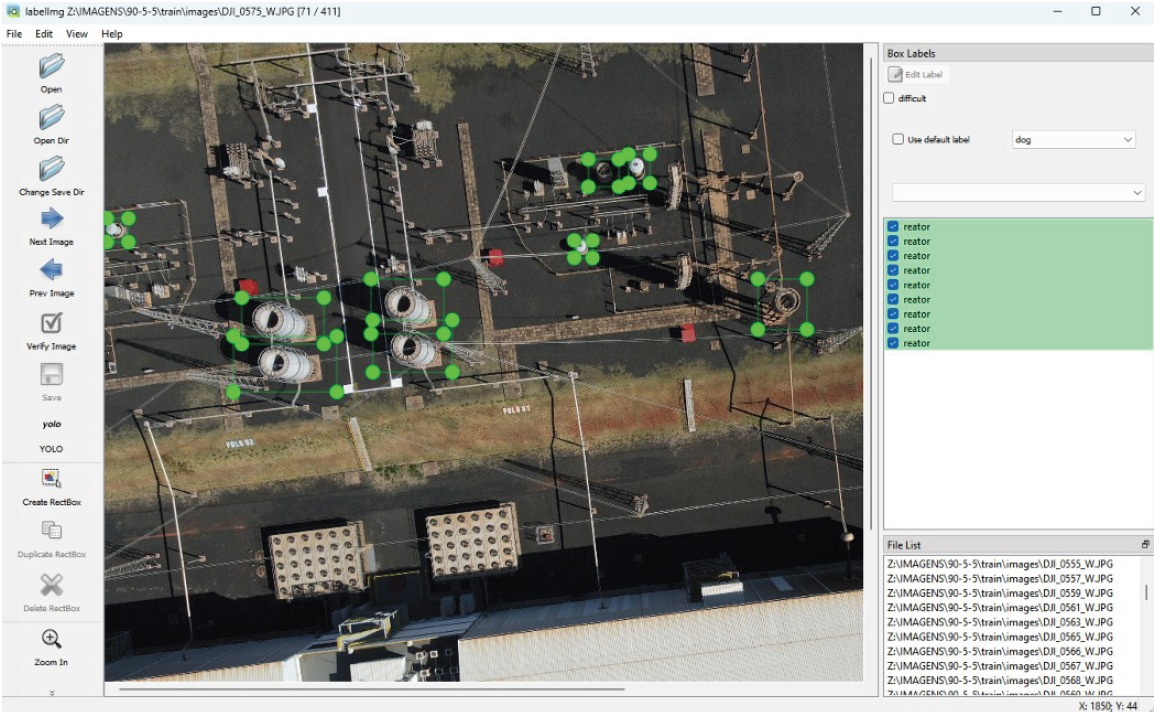
\includegraphics[width=1\linewidth]{img/cap4/marcacao.jpeg}
    \caption{LabelImg realizando a marcação de reatores de núcleo de ar}.
    \label{fig:reator-marcado}
    \end{minipage}
\end{figure}


\section{Treinamento}

\subsection{Materiais}

Todo o treinamento foi realizado em um computador pessoal, portador do Sistema Operacional Windows 11 de 64 bits, equipado com um processador x64 com 24GB de memória RAM e um processador 11th Gen Intel(R) Core (TM) i7-1165G7@2.80GHz. Os scripts da YOLOv5, YOLOv6, YOLOv7 e YOLOv8, assim como o LabelImg, foram executados no ambiente de desenvolvimento PyCharm \cite{pycharm}.

Para a implementação da automação, foi utilizado o software Unity \cite{unity}. O Unity é uma plataforma amplamente utilizada para o desenvolvimento de jogos e aplicações interativas 3D. Ele oferece um ambiente robusto e flexível, com uma vasta gama de ferramentas e recursos que facilitam a criação de experiências interativas. Além disso, o Unity permite integração com diversos outros softwares e sistemas, proporcionando um fluxo de trabalho eficiente para projetos de automação e simulação.

\section{Considerações Finais}

Neste capítulo, foram descritas as especificações do sistema desenvolvido, com ênfase nos seus principais requisitos. O próximo capítulo trará informações detalhadas sobre a implementação, além de um aperfeiçoamento das especificações iniciais.



